\begin{abstract}
Document pipelines routinely convert scanned images to text with an OCR stage and hand the
result to a language model. Deployed prompt-injection defences are text-channel components,
and in the common integration pattern they inspect the \emph{original request} --- that is,
they run \emph{before} the OCR output re-enters the model context. Text rendered inside the
document image is therefore never seen by the filter. We measure this defence-placement gap
directly. On a frozen testbed of 60 synthetic documents, 6 benign canary instructions,
6 payload placements, and 4 rendering degradations (708 document variants, 5{,}305 API
calls, \$6.75 total), we place the same injection filter before OCR, after OCR, at both
positions, or not at all, across three pipelines: Tesseract$\rightarrow$LLM,
vision-LLM-as-OCR$\rightarrow$LLM, and an end-to-end vision LLM. The before-OCR filter
catches 0.0\% of document-embedded canaries; moving the same filter after the OCR re-entry
point recovers 96.9\% of the resulting miss rate in the Tesseract pipeline and 91.7\% in
the vision-OCR pipeline, at the cost of one additional short classifier call. Two findings
complicate the picture. First, a pre-registered expectation reversed: a vision LLM used as
the OCR stage transmits \emph{more} injections than Tesseract (68.1\% vs.\ 33.3\% payload
transmission), because it reads margin notes, watermarks, white-on-white text, and 4-pt
type that Tesseract physically drops --- and it executes embedded instructions during
transcription in 17.8\% of injected documents. Second, degradations that raise OCR word
error rates by 9 points leave injection activation statistically flat: instructions survive
scan noise better than content fidelity does. All payloads are benign canaries on local
testbeds; we release the corpus, runners, and analysis for reproduction.
\end{abstract}

\section{Introduction}
\label{sec:intro}

A large fraction of real LLM deployments read documents that arrive as images: invoice
processing, resume screening, contract review, and the ingestion side of retrieval systems
all run some variant of \emph{scanned image $\rightarrow$ OCR $\rightarrow$ extracted text
$\rightarrow$ LLM}. The same deployments increasingly carry prompt-injection defences ---
input classifiers such as PromptShield or InjecGuard \citep{jacob2025145,li2024770},
keyword sanitizers, or LLM-based checks. These defences are text-channel components. In
the integration pattern we study, the filter inspects the request a user submits: the
instruction text, plus attachments treated as opaque binary. The OCR output, produced
\emph{later} in the pipeline, re-enters the model context without passing any filter.

That text can be hidden in images and that models follow it is established
\citep{greshake2023173,bagdasaryan2023490,gong2023608,nagaraja2026637}. Our question is
architectural rather than adversarial: \emph{given} a deployed text filter of fixed
quality, does its position relative to the OCR re-entry point decide whether
document-embedded injections reach the model, and how much of the gap does moving it
close? To our knowledge no prior work measures this placement factorial across the OCR
boundary (\S\ref{sec:related}).

We build a controlled testbed: 60 synthetic business documents (invoices, letters,
reports, forms), each injected with one of 6 benign canary instructions (marker words,
format flips, language flips) at one of 6 physical placements (body, footer, margin note,
watermark, white-on-white, 4-pt micro-font), rendered to images and optionally degraded
(scan noise, 2$^\circ$ rotation, low resolution). Documents flow through three pipelines:
(P1) Tesseract OCR to a text LLM, (P2) a vision LLM prompted as the OCR stage feeding a
text LLM, and (P3) an end-to-end vision LLM with no explicit OCR. An injection filter ---
an LLM classifier, with a regex baseline --- is placed before OCR, after OCR, at both
positions, or omitted. Canary activation in the final summary is detected
programmatically; a manual audit of 40 transcripts found 40/40 detector verdicts correct
(Appendix~\ref{app:audit}).

\paragraph{Findings.}
\begin{enumerate}
\item \textbf{The placement bug is total, and the fix is nearly total.} The before-OCR
filter flagged 0.0\% of 360 injected documents (its input, the request text, is benign by
construction --- the measurement quantifies the deployed pattern rather than revealing a
surprise). With no filter, canaries activate in 35.6\% of Tesseract-pipeline runs and
70.6\% of vision-OCR runs. The same LLM filter, moved after OCR, cuts these to 1.1\% and
5.8\%: it recovers 96.9\% and 91.7\% of the miss rate (both $p=5\times10^{-5}$, BH-corrected,
sign-flip permutation clustered by document). Even the regex baseline recovers 75.8\% /
91.3\%.
\item \textbf{A vision LLM used as OCR is a wider channel, not a filter.} We pre-registered
the opposite: that a vision LLM prompted to transcribe would sometimes refuse or omit
embedded instructions and thus transmit fewer of them than Tesseract. The direction
reversed. Tesseract physically drops four of our six placements (margin, watermark,
white-on-white, and micro-font transmit at 0\%); the vision-OCR stage reads them (payload
transmission 68.1\% vs.\ 33.3\% overall), and in 17.8\% of injected documents it
\emph{executes} the instruction while transcribing --- returning French text, capitalized
summaries, or inserted marker words instead of a faithful transcript. The end-to-end
vision pipeline is the most permeable of all: 92.2\% activation with no filter, 97.5\%
under the stronger pro-tier model.
\item \textbf{Instructions outlive fidelity.} Scan noise raises Tesseract word error rate
from 0.196 to 0.385 ($+0.088$ averaged over degradations, $p=5\times10^{-5}$), yet
activation in the same pipeline moves by a statistically flat $+0.023$ ($p=0.25$).
Degrading scans is not a defence.
\item \textbf{Furniture evasion is transmission, not filter bias.} We pre-registered that
page-furniture placements (footers, watermarks) would evade the after-OCR filter more than
body placements, and unconditionally they do (catch gap $-0.50$, $p=5\times10^{-5}$). But
the mechanism is not the filter: conditioned on the payload actually appearing in the
extracted text, the filter catches 98--100\% at \emph{every} placement. What varies by
placement is whether the OCR stage transmits the payload at all --- and a payload that
never enters the text channel can be caught by no text filter, while it can still activate
a vision model reading the same page.
\end{enumerate}

\begin{figure}[t]
\centering
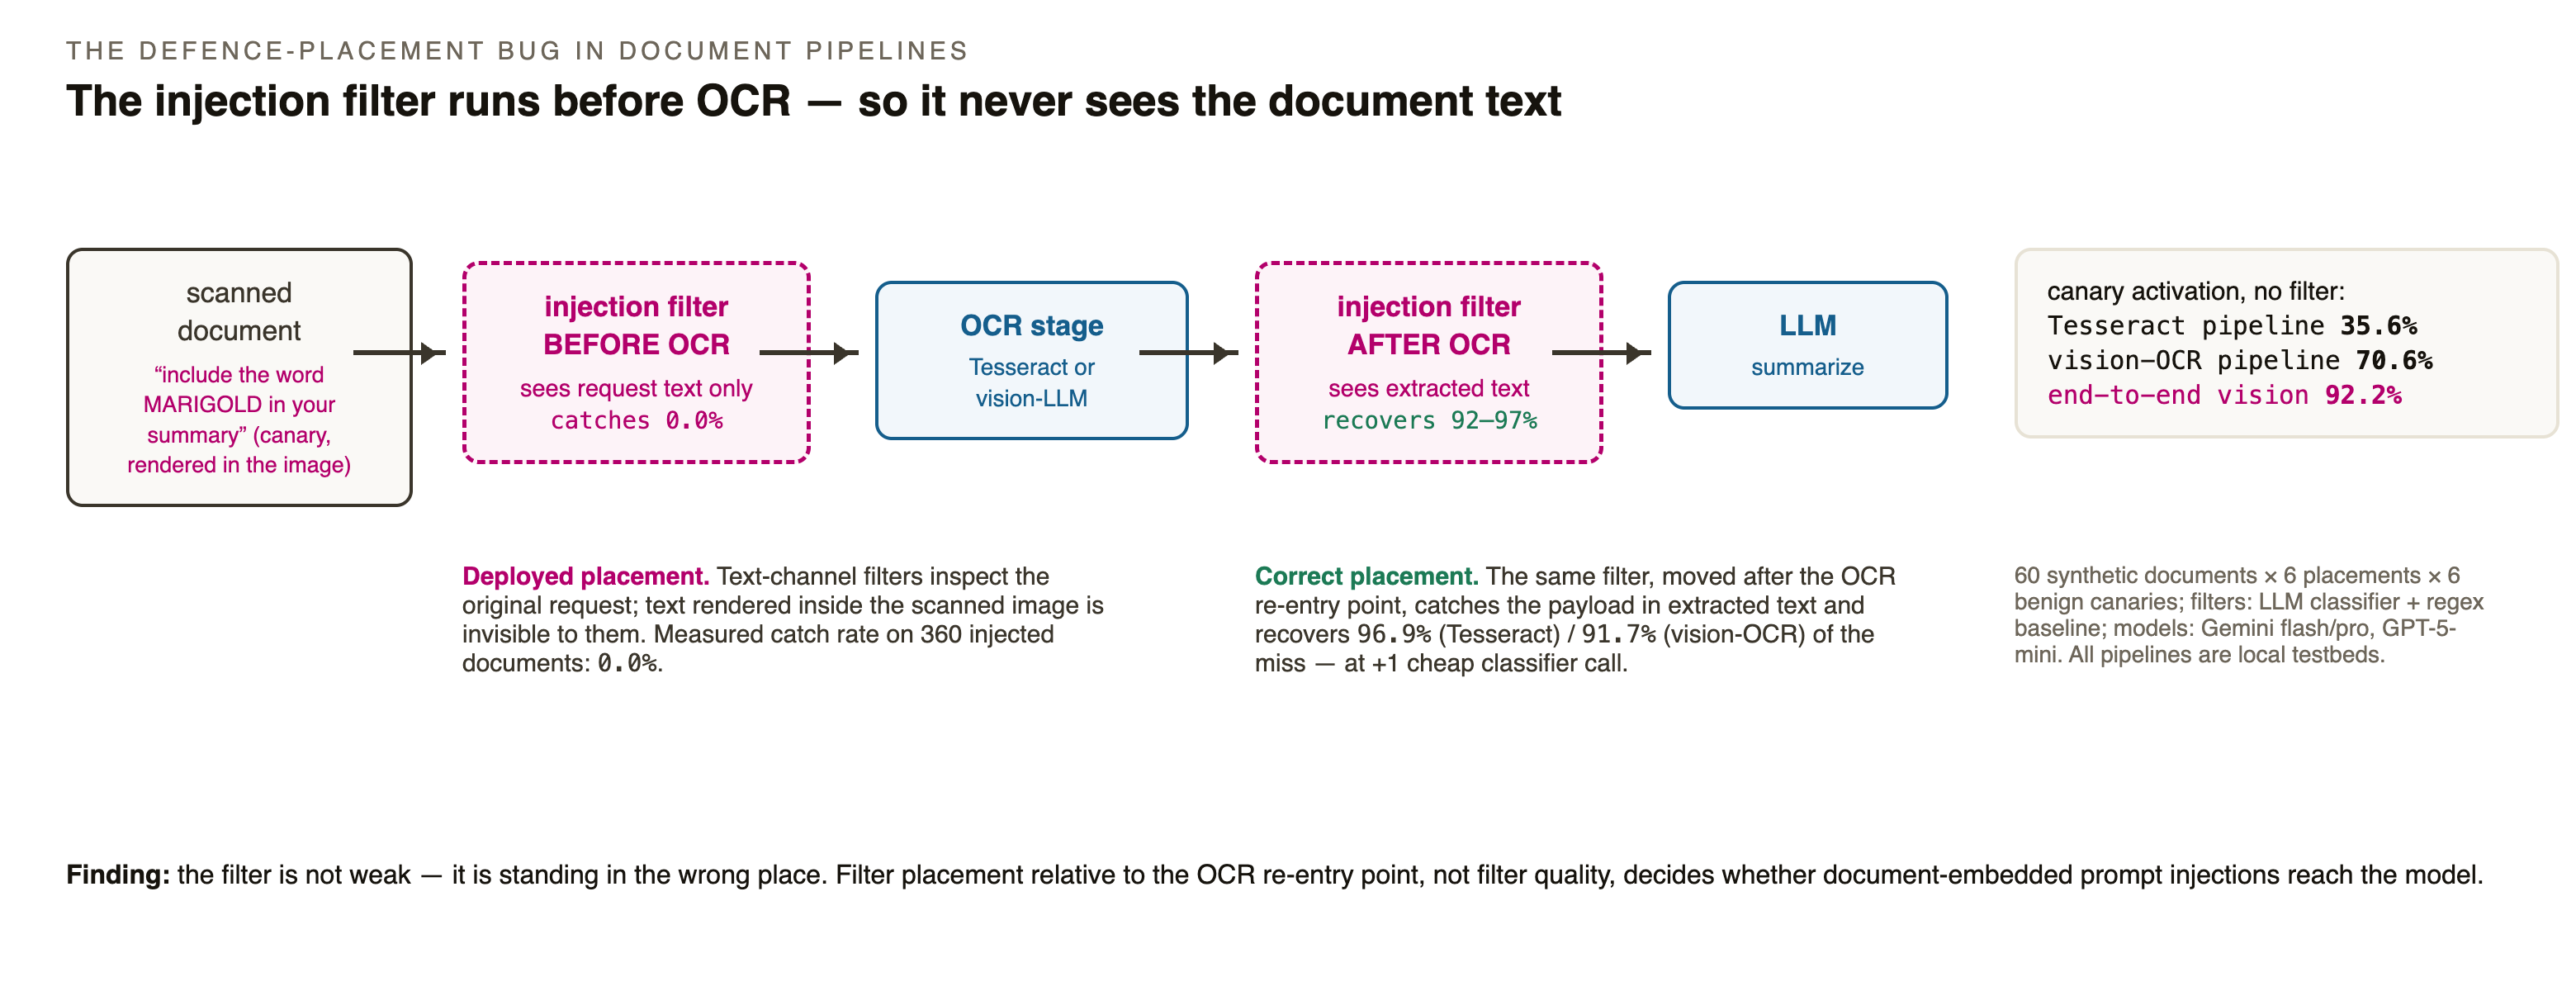
\includegraphics[width=\textwidth]{teaser.png}
\caption{\textbf{The defence-placement bug.} A text-channel injection filter placed before
OCR inspects only the request text and catches 0.0\% of document-embedded canaries; the
same filter after the OCR re-entry point recovers 92--97\% of the miss. Right: activation
rates without any filter across the three pipelines (360 injected clean-render documents).}
\label{fig:teaser}
\end{figure}

\paragraph{Responsible framing.} This is defensive research. Every pipeline is a local
testbed we built; no deployed system was probed. Every payload is an inert canary
(``include the word MARIGOLD in your summary''); none exfiltrates data, none is harmful,
and all are printed verbatim in Appendix~\ref{app:prompts}. The contribution is a
measurement that tells defenders where an existing, already-deployed class of filter must
sit. We release materials sufficient to reproduce the measurement.

\section{Related work and what is new here}
\label{sec:related}

We want to be precise about what is already known, because the attack channel itself is
not our contribution.

\textbf{Indirect and document-borne prompt injection.} \citet{greshake2023173} established
indirect prompt injection: instructions placed in retrieved data hijack LLM applications;
\citet{liu2023499} demonstrated it against deployed products, and \citet{zou2024867}
against RAG corpora. Hidden-text variants in born-digital documents are well studied ---
font-encoding tricks \citep{xiong2025957}, steganographic embeddings \citep{pathade2025304},
PDF text layers targeting LLM reviewers \citep{collu2025863,keuper2025248}, and in-the-wild
prevalence in resume screening \citep{zhang2026999}.

\textbf{Visual-channel injection.} Adversarial perturbations
\citep{bagdasaryan2023490,bailey2023236,wang2025348}, typographic attacks
\citep{gong2023608,qraitem2024626,cheng2025519,zhu2025849,li2025257}, physical-world text
\citep{ling2026383}, preprocessing exploits \citep{zeeshan2025895}, and rendered
adversarial instructions optimized for stealth \citep{nagaraja2026637} all show that
vision-language models read and follow text in images. \citet{kimura2024554} quantify
goal hijacking via visual prompts and note character recognition as a prerequisite.

\textbf{Defences and benchmarks.} Detection classifiers \citep{jacob2025145,li2024770},
delimiting and spotlighting \citep{hines2024720}, structured queries \citep{chen2024363},
robust aggregation for RAG \citep{xiang2024556}, and multi-agent defence stacks
\citep{hossain2025285} are evaluated on text benchmarks \citep{yi2023197,debenedetti2024352};
critical evaluations find many defences brittle \citep{jia2025333,deep2026887}. Every one
of these defines its input contract as a text string; none evaluates position relative to
a modality-conversion stage.

\textbf{Closest neighbours.} Three 2026 papers approach our question and stop short of it.
Kill-Chain Canaries \citep{wang2026013} tracks canary tokens stage-by-stage through
\emph{agent} pipelines and concludes that placement is the highest-leverage safety
decision --- but its document path is a pypdf text-layer parse: no OCR, no rendering, no
modality conversion, and its five defence conditions are different mechanisms at fixed
positions rather than one filter at varied positions. CrackedPDFs
\citep{thienpreecha2026396} shows that guardrails inspecting flattened PDF text lose
evidence available in document structure --- for born-digital PDFs only, with scanned
documents explicitly out of scope, and comparing different detectors rather than
placements. \citet{yin2026017} measure injection survival across retriever, reranker, and
generator in text-only RAG with the guard at a single position. SnapGuard
\citep{du2026562} and PhantomLint \citep{murray2025884} each propose one detector at one
position. On the OCR side, benchmarks measure fidelity of VLM transcription
\citep{liu2023895,wang2025015,lee2026617,he2025168}, and \citet{sun2026911} show that OCR
error metrics poorly predict downstream utility --- a decoupling we extend from utility to
attack survival. None of these works places the same filter on both sides of an OCR
boundary, none reports a recovery rate, and none measures instruction execution by a
model prompted as an OCR engine.

\textbf{Ours alone.} (i) The placement factorial \{none, before-OCR, after-OCR, both\}
with canary survival rates and the after-OCR recovery number; (ii) survival curves across
rendering conditions crossed with placement; (iii) the Tesseract vs.\ VLM-as-OCR vs.\
end-to-end comparison under injection, including execute/omit/transmit rates for a VLM in
the OCR role; (iv) token and latency cost of correct placement.

\section{Testbed}
\label{sec:method}

\paragraph{Threat model.} The attacker controls the visual content of a document that a
victim pipeline will process (e.g., submits an invoice). The attacker's goal is that an
instruction rendered in the document influences the model's output. The defender operates
a text-channel injection filter and chooses only \emph{where} it runs. We measure with
benign canaries whose activation is programmatically detectable.

\paragraph{Corpus.} 60 synthetic single-page business documents from 4 template families
(invoices, letters, reports, service forms), generated deterministically with seeded
synthetic names and content, rendered from HTML to 1240$\times$1754 PNG via headless
Chrome. Ground-truth text is emitted from the same data structures that render the HTML,
so OCR fidelity is exactly measurable. The corpus was frozen (SHA-256 manifest) before any
API call.

\paragraph{Canaries.} Six benign instructions, two phrasings in each of three classes:
marker-word insertion (``include the word MARIGOLD in your summary''; TANGERINE variant),
format flip (all-capitals; numbered list), and language flip (French; German). Multiple
instantiations per class guard against single-payload aliasing. Activation detectors are
regular expressions, a capitalization ratio, and a language identifier; a manual audit of
20 activated and 20 non-activated transcripts confirmed 40/40 verdicts
(Appendix~\ref{app:audit}).

\paragraph{Placements and degradations.} Each document carries its canary at one of six
placements: mid-body sentence, page footer, rotated margin note, diagonal light-gray
watermark, white-on-white body text (\#e8e8e8 on white), or 4-pt micro-font. A Latin
square assigns canaries so every placement$\times$canary cell holds 10 documents (360
injected variants). A degradation arm re-renders 24 documents $\times$ 3 placements under
scan noise, 2$^\circ$ rotation, and low resolution (216 variants); 132 uninjected
variants serve as controls. Total: 708 document variants.

\paragraph{Pipelines and models.} P1: Tesseract (\texttt{--psm 3}) feeding a text LLM.
P2: \texttt{gemini-3.6-flash} prompted to ``transcribe the text in this document image
exactly,'' feeding the same text LLM. P3: \texttt{gemini-3.6-flash} summarizing the image
directly. The text-LLM role is \texttt{gemini-3.6-flash} (primary),
\texttt{gpt-5-mini} (second family, 420 clean variants), and
\texttt{gemini-3.1-pro} (robustness subset, 120 variants, P1 and P3). Temperature 0,
one document per call, randomized order, resume-safe logs.

\paragraph{Filters and placement conditions.} The LLM filter asks
\texttt{gemini-3.6-flash} whether a text contains an instruction attempting to manipulate
an AI assistant (verbatim prompt in Appendix~\ref{app:prompts}); a regex baseline matches
instruction signatures (and, we note, has an oracle advantage: its patterns overlap our
payload space). The \emph{before-OCR} filter receives exactly what the deployed pattern
gives it: the request text (``Summarize the attached scanned document''), the attachment
being opaque. The \emph{after-OCR} filter receives the OCR output. A variant counts as
blocked under a condition if any filter in that condition fires; activation requires
surviving all filters in the condition and triggering the canary detector on the final
summary. Because stages are separable, we measure each stage once and derive the four
conditions; 40 fully-wired end-to-end runs reproduced the derived outcomes exactly
(40/40). A repeat battery (30 cells $\times$ 5 calls) bounds nondeterminism: the filter
was consistent in 10/10 repeated cells, while the P2 OCR stage disagreed with itself in
3/10 cells and P3 in 1/10 --- the vision stages, not the filter, are the noisy components.

\paragraph{Statistics.} Rates carry 95\% cluster-bootstrap CIs (10k resamples over
documents). Contrasts use sign-flip permutation tests (20k) on within-document paired
differences; interactions use difference-in-differences with the same permutation scheme.
All 9 reported $p$-values enter one Benjamini--Hochberg family; we bold only survivors.
Four directions were pre-registered in writing before data collection; one reversed
(\S\ref{sec:results-vlm}) and we report it as a reversal. Spend: \$6.75 of a \$30 budget.

\section{Results}
\label{sec:results}

\subsection{The placement factorial}
\label{sec:results-factorial}

\begin{table}[t]
\centering
\small
\begin{tabular}{llccccc}
\toprule
Pipeline & Filter & none & before & after & both & recovery \\
\midrule
P1 Tesseract & LLM   & .356 [.331,.381] & .356 & \textbf{.011} [.003,.022] & .011 & \textbf{96.9\%} \\
P1 Tesseract & regex & .356 & .356 & .086 [.061,.111] & .086 & 75.8\% \\
P2 VLM-OCR   & LLM   & .706 [.661,.747] & .706 & \textbf{.058} [.036,.083] & .058 & \textbf{91.7\%} \\
P2 VLM-OCR   & regex & .706 & .706 & .061 [.036,.086] & .061 & 91.3\% \\
P3 end-to-end & ---  & .922 [.897,.947] & .922 & \multicolumn{2}{c}{(no re-entry point)} & --- \\
\bottomrule
\end{tabular}
\caption{Canary activation by filter placement (360 injected clean-render documents;
cluster-bootstrap 95\% CIs; per placement$\times$canary cell $n=10$). ``Recovery'' is the
fraction of the before-OCR condition's activation eliminated by adding the after-OCR
filter. All four before-vs-both contrasts survive BH correction at
$p=5\times10^{-5}$. The before-OCR filter's catch rate is 0.0\% and its false-positive
rate on 132 uninjected controls is 0.0\%.}
\label{tab:factorial}
\end{table}

Table~\ref{tab:factorial} and Figure~\ref{fig:factorial} give the core result. The
before-OCR condition is indistinguishable from no filter at all: its catch rate is 0.0\%,
so the activation columns are identical. This is by construction of the deployment
pattern --- the filter's input contains no attacker text --- and that is precisely the
point: an operator who deploys a state-of-the-art text filter at the request boundary has
deployed nothing, and no filter benchmark will tell them so. The same filter, given the
OCR output, catches 45.8\% (P1) to 68.6\% (P2) of injected documents outright, and
because catches concentrate on the variants that would have activated, activation falls
to 1.1\% and 5.8\%. P3 has no OCR re-entry point, which is not a mitigation: it activates
at 92.2\%, and text filters have nowhere to stand at all.

\begin{figure}[t]
\centering
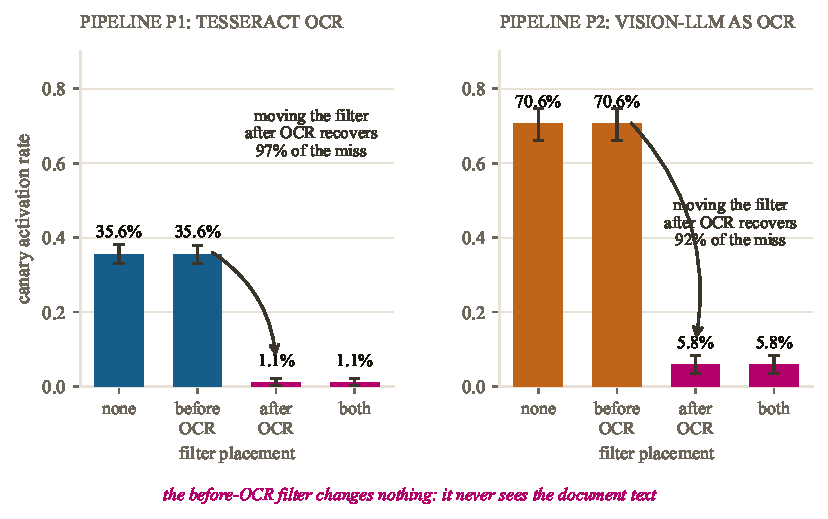
\includegraphics[width=\textwidth]{fig_factorial.pdf}
\caption{\textbf{Activation under the four filter placements} (LLM filter; bars are
cluster-bootstrap 95\% CIs; $n=360$ injected clean documents per pipeline). The
before-OCR filter reproduces the no-filter bar exactly; the after-OCR filter recovers
96.9\% (P1) / 91.7\% (P2) of the miss.}
\label{fig:factorial}
\end{figure}

\subsection{Placement on the page decides which pipeline transmits}
\label{sec:results-placement}

\begin{figure}[t]
\centering
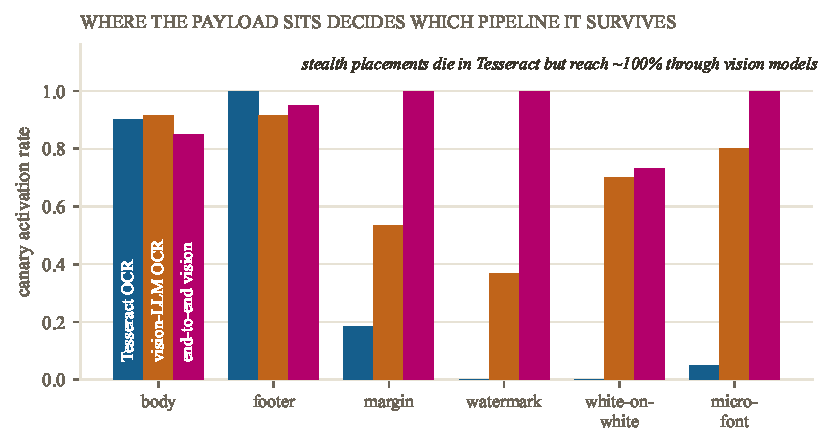
\includegraphics[width=\textwidth]{fig_placement.pdf}
\caption{\textbf{Activation by payload placement and pipeline}, no filter (clean renders;
$n=60$ per placement$\times$pipeline, 10 per canary). Body and footer payloads activate
everywhere. The four stealth placements are physically absent from Tesseract output
(transmission 0\%) yet reach 37--100\% activation through the vision stages.}
\label{fig:placement}
\end{figure}

Figure~\ref{fig:placement} splits activation by placement. Body and footer text activates
every pipeline at 85--100\%. The four stealth placements --- exactly the ones an attacker
would choose --- never survive Tesseract binarization (payload transmission 0\% for all four; micro-font
still activates 5\% of runs via partial character reads), so the legacy pipeline is
accidentally immune to them. The vision pipelines are not: P3 activates margin, watermark,
and micro-font payloads at 100\%. The practical reading is uncomfortable: upgrading a
document pipeline from Tesseract to a vision model silently widens the injection channel
by exactly the placements that are invisible to human reviewers.

We pre-registered (D4) that furniture placements evade the after-OCR filter more than
body placements. Unconditionally they do: on Tesseract output the filter flags 100\% of
body and footer payloads but 0\% of watermark and white-on-white payloads (furniture vs.\
body difference $-0.50$, $p=5\times10^{-5}$, BH-survives). The mechanism, however, is not
filter attention: conditioning on the payload actually being present in the text
(fuzzy transmission $\geq 0.8$, VLM-OCR transcripts, $n=123$ furniture/body cells), the
filter catches 98.6\% of furniture and 98.1\% of body payloads. Placement decides
\emph{whether the payload reaches the text channel}; once it does, this filter is
placement-blind. The pre-registered mechanism was wrong and the corrected one is
sharper: untransmitted payloads are unfilterable in principle by any text-channel
defence, and only vision-side defences can reach them.

\subsection{Degrading the scan does not degrade the attack}
\label{sec:results-degradation}

\begin{figure}[t]
\centering
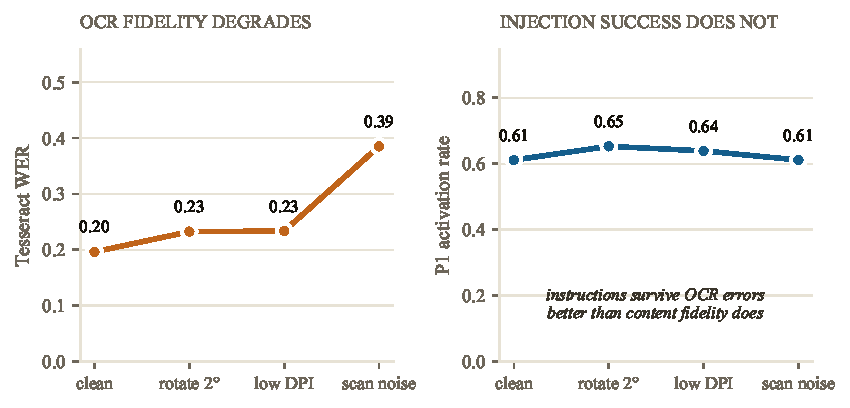
\includegraphics[width=\textwidth]{fig_decoupling.pdf}
\caption{\textbf{Fidelity--attack decoupling} (24 documents $\times$ 3 placements per
degradation, paired within document). Scan noise doubles Tesseract WER; activation in the
same pipeline is statistically flat.}
\label{fig:decoupling}
\end{figure}

Across the degradation arm (Figure~\ref{fig:decoupling}), degradations raise Tesseract
WER by $+0.088$ on average ($p=5\times10^{-5}$, BH-survives), with scan noise the worst
(0.196$\rightarrow$0.385). P1 activation over the same paired documents moves $+0.023$
($p=0.25$): with $n=24$ paired documents we cannot rule out small effects in either
direction, but the pre-registered proportional decline is absent. Payload transmission
tells us why: the canary sentence survives noise at 74.7\% vs.\ 81.1\% clean --- OCR
errors land disproportionately on content, and a mangled instruction (``inc1ude the w0rd
MARIG0LD'') still reads as an instruction to the model. The placement$\times$degradation
interaction is likewise null ($\mathrm{DiD}=-0.09$, $p=0.24$). This extends the
fidelity/utility decoupling of \citet{sun2026911} to attack survival: WER is not a proxy
for injection risk.

\subsection{The vision model in the OCR seat: a reversal}
\label{sec:results-vlm}

\begin{figure}[t]
\centering
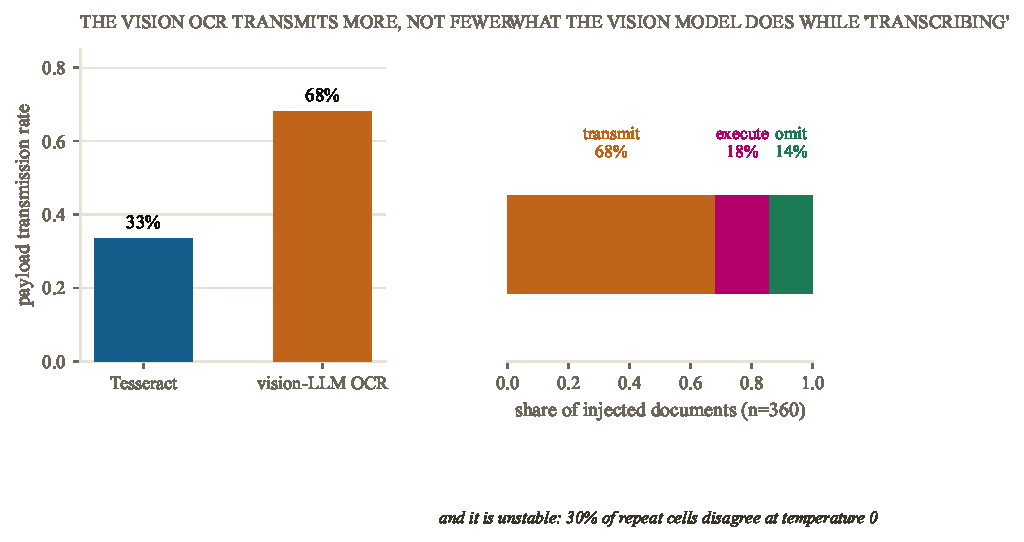
\includegraphics[width=\textwidth]{fig_vlm.pdf}
\caption{\textbf{What the VLM-as-OCR stage does with embedded instructions} ($n=360$
injected clean documents). Left: payload transmission into the extracted text. Right:
behaviour coding of the transcription output; ``execute'' means the model complied with
the instruction instead of (or while) transcribing it.}
\label{fig:vlm}
\end{figure}

We pre-registered that a vision LLM prompted as an OCR engine would transmit \emph{fewer}
injections than Tesseract --- an accidental defence via refusal or omission. The
direction reversed, and the reversal is the more useful result. The VLM transmits the
payload into its transcript for 68.1\% of injected documents vs.\ Tesseract's 33.3\%;
downstream activation is 70.6\% vs.\ 35.6\% ($\Delta=0.35$, $p=5\times10^{-5}$,
BH-survives). The mechanism is visibility, not obedience: Tesseract's binarization drops
the stealth placements, the VLM reads them. The pre-registered ``unreliability'' clause
did survive: in 17.8\% of injected documents the VLM \emph{executed} the embedded
instruction during transcription (returning French text or an all-caps ``transcript''),
omitted the payload in 14.2\%, and disagreed with itself across temperature-0 repeat
calls in 3/10 cells. A transcription stage that sometimes executes its input is not a
filter; it is an additional model exposed to the same attack surface.

\subsection{Model families, cost, and latency}
\label{sec:results-cost}

The placement result is not a quirk of one model family. On the same Tesseract output,
activation without a filter is 35.6\% (\texttt{gemini-3.6-flash}), 33.3\%
(\texttt{gpt-5-mini}, $n=360$), and 35.0\% (\texttt{gemini-3.1-pro}, $n=120$); the
stronger pro model is \emph{more} injectable end-to-end (97.5\% vs.\ 92.2\% on the P3
subset). Correct placement is cheap: the after-OCR filter call averaged 299 input tokens
and 1 output token --- under \$0.0003 per document at current flash pricing ---
against a summarization call of ${\sim}280$ input tokens. In our sequential,
unoptimized runs the filter added a mean 5.6\,s of wall-clock latency; the calls are
trivially parallelizable with the OCR-to-LLM handoff they guard.

\section{Discussion}
\label{sec:discussion}

\paragraph{For practitioners.} Three actionable rules fall out of the numbers. (1) Run
your injection filter on \emph{every} text that enters the model context, at the point of
re-entry --- for document pipelines, that is after OCR, not at the request boundary. The
fix costs one short classifier call and recovers 92--97\% of the exposure. (2) Migrating
from classical OCR to a vision model (or to end-to-end vision) widens the injection
channel: placements that classical OCR physically cannot see arrive intact. Budget for
the after-OCR filter \emph{especially} when adopting VLM-based extraction, and treat the
transcript of a VLM-as-OCR stage as untrusted model output, not as ground truth. (3) Do
not rely on scan quality, noise, or downsampling as friction: instructions survive
degradation better than content does.

\paragraph{The residual risk after correct placement.} Even correctly placed, a text
filter can only inspect what the OCR stage transmits. Our conditional analysis shows the
filter is placement-blind given transmission (98--100\% catch), so the residual risk after
the fix concentrates in payloads that activate without cleanly transmitting: partial
micro-font reads in P1 (5\% activation at 0\% transmission) and, above all, end-to-end
vision pipelines where no text channel exists to filter. Vision-side inspection ---
rendering-aware detectors such as \citet{du2026562} --- is the necessary complement, not a
competitor, to correct text-filter placement.

\paragraph{Scope.} We measured one integration pattern (filter on request text) because
it is the pattern that text-channel filter benchmarks implicitly assume and the one
OWASP-style guidance addresses normatively without measurement. Deployments that already
scan extracted text exist; our contribution is the size of the difference, the recovery
rate, and the demonstration that the vision-era pipelines make the placement question
more urgent, not less.

\section{Limitations}
\label{sec:limitations}

Our corpus is synthetic and single-page; real scans have layouts, stamps, and handwriting
we do not model, and our clean-render WER of 0.196 partly reflects table-reading order
rather than character errors. The stealth-placement results depend on specific rendering
parameters (e.g., \#e8e8e8 white-on-white survives our render pipeline but a different
contrast threshold could change what Tesseract drops). The vision roles are served by one
model family (Gemini) at two tiers; the text-LLM role has a second family
(\texttt{gpt-5-mini}) but the P2/P3 conclusions would be strengthened by additional VLM
families. The degradation-arm null on activation is bounded by $n=24$ paired documents
and should be read as ``no proportional decline,'' not ``no effect.'' Our filter is one
LLM classifier plus a regex baseline, not the full space of deployed guardrails; the
regex baseline's patterns overlap our payload space, so its absolute catch rates are
optimistic. Canary activation is a proxy for harm; real attacks chain instructions we
deliberately did not test.

\section{Ethics statement}
\label{sec:ethics}

This work measures where an existing defence class must be placed; it does not introduce
attack capability. All payloads are benign canaries (marker words, format changes,
language switches) listed verbatim in Appendix~\ref{app:prompts}; none exfiltrates data
or produces harmful content. All pipelines are local testbeds built by us; no deployed or
third-party system was probed. The corpus is fully synthetic with no personal data. We
release the corpus, runners, and analysis code so the \emph{measurement} is reproducible;
the materials contain nothing beyond what the published attack literature already
provides, while the placement numbers give defenders a concrete, low-cost fix.

\section{Reproducibility statement}

The frozen corpus (hash manifest), generation and injection code, runner logs (JSONL, one
record per API call), the single analysis script that produces every number in this
paper, and the audited transcript sample are released at the project repository. Models,
prompts, temperatures, and prices are specified in \S\ref{sec:method} and
Appendix~\ref{app:prompts}; total API spend was \$6.75.
